%%%%%%%%%%%%%%%%%%%%%%%%%%%%%%%%%%%%%%%%%
% Professional Formal Letter
% LaTeX Template
% Version 1.0 (28/12/13)
%
% This template has been downloaded from:
% http://www.LaTeXTemplates.com
%
% Original author:
% Brian Moses (http://www.ms.uky.edu/~math/Resources/Templates/LaTeX/)
% with extensive modifications by Vel (vel@latextemplates.com)
%
% License:
% CC BY-NC-SA 3.0 (http://creativecommons.org/licenses/by-nc-sa/3.0/)
%
%%%%%%%%%%%%%%%%%%%%%%%%%%%%%%%%%%%%%%%%%

% may not be compatible with rest of template
% \documentclass[journal=jpcbfk,manuscript=article]{achemso}

%----------------------------------------------------------------------------------------
%	PACKAGES AND OTHER DOCUMENT CONFIGURATIONS
%----------------------------------------------------------------------------------------

%\documentclass[11pt,a4paper,draft]{letter} % Specify the font size (10pt, 11pt and 12pt) and paper size (letterpaper, a4paper, etc) 
\documentclass[11pt,a4paper]{letter} % Specify the font size (10pt, 11pt and 12pt) and paper size (letterpaper, a4paper, etc) 
\usepackage{letterbib}
\usepackage{graphicx} % Required for including pictures
\usepackage{microtype} % Improves typography
\usepackage{fancyhdr}
\usepackage[T1]{fontenc} % Required for accented characters
\usepackage[sort&compress,numbers,super]{natbib}
\usepackage{caption}
\usepackage{newfloat}
\usepackage{float}
\usepackage{url}
\usepackage{color}
\usepackage{soul}
\usepackage[svgnames]{xcolor}
\usepackage{framed}
\usepackage{calligra}
\usepackage{fp}
\FPset\marginWidth{0.7}	% margin width (all sides) in inches
\usepackage[margin=\marginWidth in]{geometry}
\usepackage{marginfix}
\usepackage[colorlinks=true,
            linkcolor=blue,
            urlcolor=blue,
            citecolor=blue]{hyperref}
            

% Create a new command for the horizontal rule in the document which allows thickness specification
\makeatletter

\def\vhrulefill#1{\leavevmode\leaders\hrule\@height#1\hfill \kern\z@}
\makeatother

%more new commands and definitions
%\newcommand*{\rood}[1]{\color{red}{#1}}
\newcommand*{\rood}[1]{{\color{red}{#1}}}
\newcommand*{\noteg}[1]{\textcolor{green}{[[#1]]}}		% notes 

\newcommand*{\blauw}[1]{\color{blue}{#1}}
\newcommand*{\groen}[1]{\color{green}{#1}}
\newcommand{\hlc}[2][yellow]{{\sethlcolor{#1}\hl{#2}}}
\newcommand{\scripty}[1]{\ensuremath{\mathcalligra{#1}}}

% code for custom comments
\usepackage{tikz}
\usepackage{xcolor}
\usepackage{mathtools}

% markers (black, blue, brown, cyan, darkgray, gray, green, lightgray, lime, magenta, olive, orange, pink, purple, red, teal, violet, white, yellow, more: https://en.wikibooks.org/wiki/LaTeX/Colors)
\newcommand{\marker}[3]{
  \tikz[baseline=(X.base)]{
    \node [fill=#1!40,rounded corners] (X) {#2:};
  }
  {\color{#1!80!black}#3}
}
\newcommand{\khb}[1]{\marker{teal}{KHB}{#1}}  % Kathy Breen
\newcommand{\replyhead}{\textbf{Author Reply: }}

\newfloat{figure}{h}{lot}
\floatname{figure}{Figure}
\newfloat{sfigure}{h}{lot}
\floatname{sfigure}{Figure}
\newfloat{lfigure}{h}{lot}
\floatname{lfigure}{Figure}

\definecolor{shadecolor}{named}{LightGray}

\DeclareMathAlphabet{\mathcalligra}{T1}{calligra}{m}{n}
\DeclareFontShape{T1}{calligra}{m}{n}{<->s*[2.2]callig15}{}

\renewcommand{\thesfigure}{S\arabic{sfigure}}
\renewcommand{\thelfigure}{\Alph{lfigure}}

%-----------------------------------------------------------------------------
% HEADER/FOOTER INFO
%-----------------------------------------------------------------------------
%\pagestyle{fancy}
\fancyhf{}
%\cfoot{\textit{telephone} 217-333-1441 $\bullet$ \textit{fax} 217-333-2736 $\bullet$ \textit{email} matse@illinois.edu}
\cfoot{\thepage}

%----------------------------------------------------------------------------------------
%	SENDER INFORMATION
%----------------------------------------------------------------------------------------

\def\Who{Andrew L. Ferguson} % Your name
\def\What{, PhD} % Your title
\def\Where{Pritzker School of Molecular Engineering\\University of Chicago} % Your department/institution
\def\department{Pritzker School of Molecular Engineering}
\def\institution{University of Chicago}
\def\Address{5640 South Ellis Avenue} % Your address
\def\CityZip{Chicago, IL 60637} % Your city, zip code, country, etc
\def\Email{e:~\url{andrewferguson@uchicago.edu}} % Your email address
\def\TEL{p:~(773)~702-5950} % Your phone number
\def\URL{w:~\url{www.ferglab.com}} % Your URL
\def\titleone{Associate Professor\\ Deputy Dean for Equity, Diversity, and Inclusion}

%----------------------------------------------------------------------------------------
%	HEADER AND FROM ADDRESS STRUCTURE
%----------------------------------------------------------------------------------------

\FPmul\tmp{2}{\marginWidth}	% computing institution logo indent based on margin width
\FPsub\logoIndent{7.55}{\tmp}

\address{

\includegraphics[width=3.5in]{UChicago_PME_logo.png} % Include the logo of your institution
%\hspace{\logoIndent in} % Position of the institution logo, increase to move left, decrease to move right
\hspace{2.8in} % Position of the institution logo, increase to move left, decrease to move right
\vskip -0.82in~\\ % Position of the text in relation to the institution logo, increase to move down, decrease to move up
\Large\hspace{0.75in} \hfill ~\\[0.05in] % First line of institution name, adjust hspace if your logo is wide
\hspace{0.75in} \hfill \normalsize % Second line of institution name, adjust hspace if your logo is wide
\makebox[0ex][r]{\bf \Who \What }\hspace{0.65in} % Print your name and title with a little whitespace to the right
~\\[-0.11in] % Reduce the whitespace above the horizontal rule
\hspace{0in}\vhrulefill{1pt} \\ % Horizontal rule, adjust hspace if your logo is wide and \vhrulefill for the thickness of the rule
\hspace{\fill}\parbox[t]{4in}{ % Create a box for your details underneath the horizontal rule on the right
\footnotesize % Use a smaller font size for the details
%\Who \\  % Your name, all text after this will be italicized
%\\
\titleone
%\titletwo\\
%\titlethree\\
%\titlefour\\
\vskip 0.05in
\department\\ % Your department
\institution\\ % Your institution
\Address\\ % Your address
\CityZip
\vskip 0.05in
\TEL\\ % Your phone number
\Email\\ % Your email address
\URL\\ % Your URL
}
\hspace{-1.4in} % Horizontal position of this block, increase to move left, decrease to move right
\vspace{-1in} % Move the letter content up for a more compact look
}

%----------------------------------------------------------------------------------------
%	TO ADDRESS STRUCTURE
%----------------------------------------------------------------------------------------

\FPmul\tmp{2}{\marginWidth}	% computing date indent based on margin width
\FPsub\dateIndent{4.15}{\tmp}

\def\opening#1{\thispagestyle{empty}
{\centering\fromaddress \vspace{1.1in} \\ % Print the header and from address here, add whitespace to move date down
%
\hspace*{4.15 in}\today\hspace*{\fill}\par
} % Print today's date, remove \today to not display it
{\raggedright \toname \\ \toaddress \par} % Print the to name and address
\vspace{0.05in} % White space after the to address
\noindent #1 % Print the opening line
% Uncomment the 4 lines below to print a footnote with custom text
%\def\thefootnote{}
%\def\footnoterule{\hrule}
%\footnotetext{\hspace*{0.18\textwidth}{Telephone 217-333-1441 $\bullet$ Fax 217-333-2736 $\bullet$ email matse@illinois.edu\footnotesize \hspace{3cm} \thepage}}
%\def\thefootnote{\arabic{footnote}}
}

%----------------------------------------------------------------------------------------
%	SIGNATURE STRUCTURE
%----------------------------------------------------------------------------------------

\signature{\Who \What} % The signature is a combination of your name and title

\long\def\closing#1{
\vspace{0.1in} % Some whitespace after the letter content and before the signature
\noindent % Stop paragraph indentation
%\hspace*{\longindentation} % Move the signature right
%\parbox{\indentedwidth}{\raggedright
#1 % Print the signature text
\vskip 0.0in
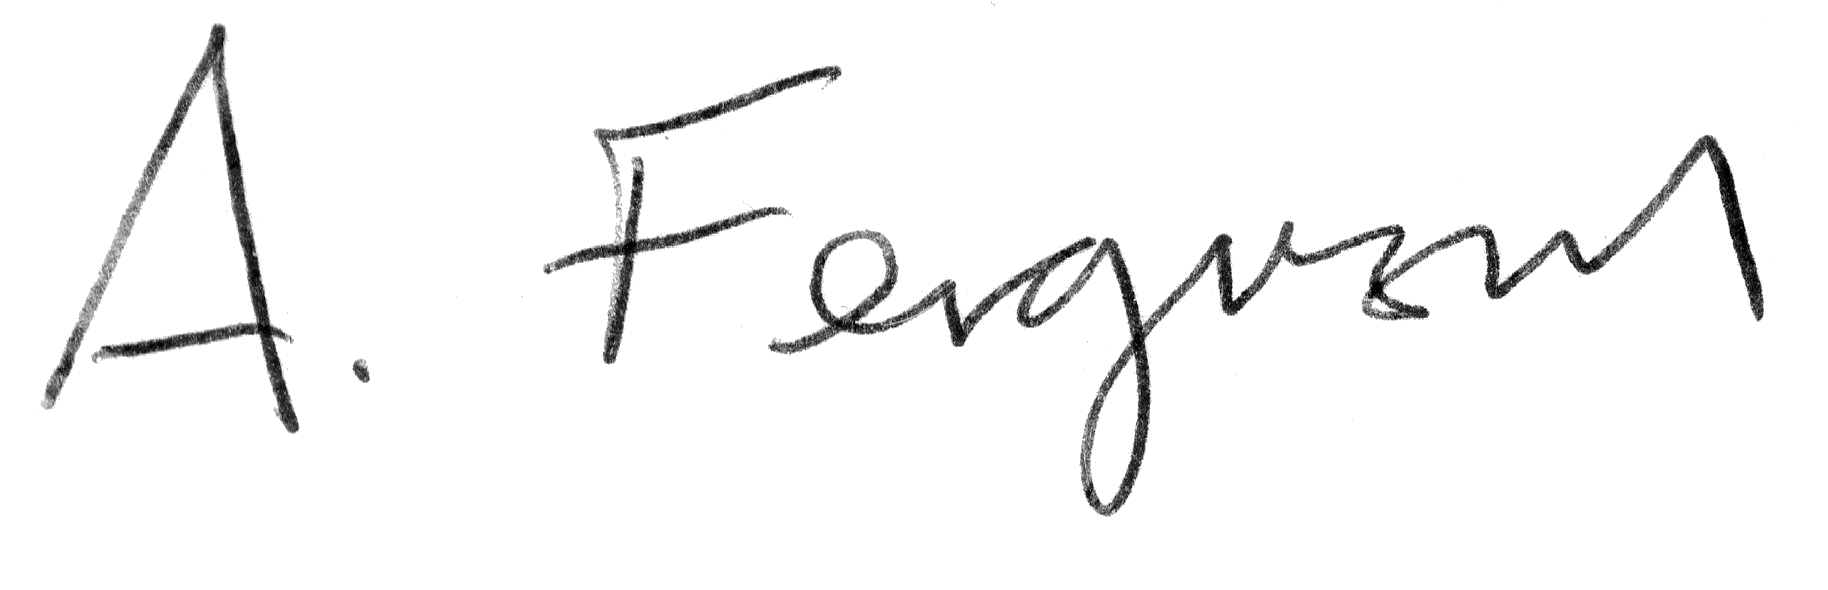
\includegraphics[width=0.2\textwidth]{signature_720}
%\vskip 0.65in % Whitespace between the signature text and your name
\\
\noindent
\fromsig
\vskip -0.05in
\titleone\\
\department\\
\institution\\
\vskip -0.1in
\noindent cc: M.S.~Jones, B.~Ashwood, A.~Tokmakoff
}

%----------------------------------------------------------------------------------------

\begin{document}

%----------------------------------------------------------------------------------------
%	TO ADDRESS
%----------------------------------------------------------------------------------------

\begin{letter}
{
Prof.\ Hanadi Sleiman \\
Associate Editor, \textit{The Journal of the American Chemical Society}
}

%----------------------------------------------------------------------------------------
%	LETTER CONTENT
%----------------------------------------------------------------------------------------

\opening{Dear Prof.\ Sleiman}

Thank you for your 23-Jul-2020 message regarding our article “Molecular Latent Space Simulators” assigned ID SC-EDG-07-2020-003635. We thank you for handling our submission and the anonymous reviewers for their careful reading and critical assessment of our work.

We reproduce below the full text of the reviewer comments in blue along with our responses, reproduction of the changes made to our manuscript, and the locations of these edits. The modifications within our revised submission in response to the reviewer comments are indicated in red text. 

In light of these changes, we hope that our revised submission is suitable for publication in Chemical Science.

\closing{Yours Sincerely}

\end{letter}

%----------------------------------------------------------------------------------------

\clearpage
\newpage

\noteg{My notes and questions are all in green. The rest of the color scheme is the same as the example you sent me. For most comments I have attempted some change in this doc but have not changed anything major in the actual manuscript or tracked version (manuscript\_marked\_up.tex) yet. In some places I have proposed a couple options but did not want to delve to deep in case I'm going down the wrong path.} 

\begin{shaded}
\textbf{Response to Reviewer \# 1}
\end{shaded}

\textcolor{blue}{In the manuscript “Determining sequence-dependent DNA oligonucleotide hybridization and dehybridization mechanisms using coarse-grained molecular simulation, Markov state models, and infrared spectroscopy”, Jones et al. provide a well-designed and compelling study of DNA hybridization kinetics and dynamics that succinctly encompasses both experiment and theory. They demonstrate that the coarse-grained model of DNA, 3SPN.2, can not only well-reproduce the relative kinetic rates of sequence-dependent hybridization but also can reveal critical insights into their physical underpinnings. These insights are driven by the use of state-of-the-art applications of machine learning to Markov state model construction and well-validated with temperature jump infrared spectroscopy. In particular, the demonstration of how the placement of two G:C base pairs within the sequence can dramatically affect the energy landscape is truly impactful for the design of DNA sequences with desired properties. We believe this work is well suited for JACS publication after the Authors address a few major and minor points.}

\textbf{Author Reply:}   We thank the reviewer for their close reading of the manuscript and are pleased they find it significant to JACS readers.

\textcolor{blue}{Major point.
1)      Many of the core conclusions about the hybridization and dehybridzation mechanisms are based on the designation of the relevant metastable states as H, 5S2, 3S2, 5S4, F4, and D. While the authors do an excellent job of demonstrating that 2-6 state models provide an accurate description of the dynamics, in the current form, the paper does not provide sufficient evidence to support their chosen representative microstates and associated nomenclature (the only evidence being the ‘representative’ structures shown in Figures 2A, C). A given macrostate represents an ensemble of microstates and it should be demonstrated that a significant fraction of the microstates that have a high probability of belonging to a particular macrostate share the same or similar base-pairing pattern. This would better justify how the authors chose to describe these states as 5S2, 3S2, etc., and provide the reader with more confidence that the mechanisms follow from the simulations. At the least, the authors should describe how the representative microstates (depicted in Figure 2A, C) were obtained.
}

\textbf{Author Reply:}   We acknowledge that the designation of states is crucial to the core conclusions of the manuscript and that some information regarding state definitions and representative structures was unclear.

\noteg{I think this comment is really getting at why the cartoon representations are appropriate to describe the state as a whole and is less concerned with how we obtained the molecular rendering. I've tried to address both aspects below and can add more detail the first figure or choose a different kind of representation.}

When defining macrostates, we both visually inspected configurations and compared distributions along a variety of structural features.  During the analysis process, we have found that two distance features in particular allow for interpretable visualization of each of the seven macrostate. Specifically, these features correspond to the reciprocal mean distance between 2-base-shifted base pairs in the 5$\prime$ and 3$\prime$ directions. These features highlight not only shifted states in both directions, but also a distinct frayed regions between the H and D wells. We have visualized these features below (Figure \ref{fig:macrostate_colors_FES}), and use the PyEMMA free energy function to plot the distribution of each macrostate/sequence on the low dimensional feature representation. Each color map corresponds to a different macrostate according to the legend, and lighter regions indicate a higher probability at equilibrium (lower free energy). We agree with the reviewer that it is important for readers to understand the physical definitions and distributions of each macrostate and its associated microstates, and we have added this figure to the supplemental information.

%In order to demonstrate that configuration in a given macrostates are well-defined by the representations in figure 2, we show the distribution of several structural metrics for each macrostate and sequence combination. These metrics are a collection of mean intermolecular distance that we have found work well to differentiate between states. 

\begin{figure}[ht!]
	\begin{center}
        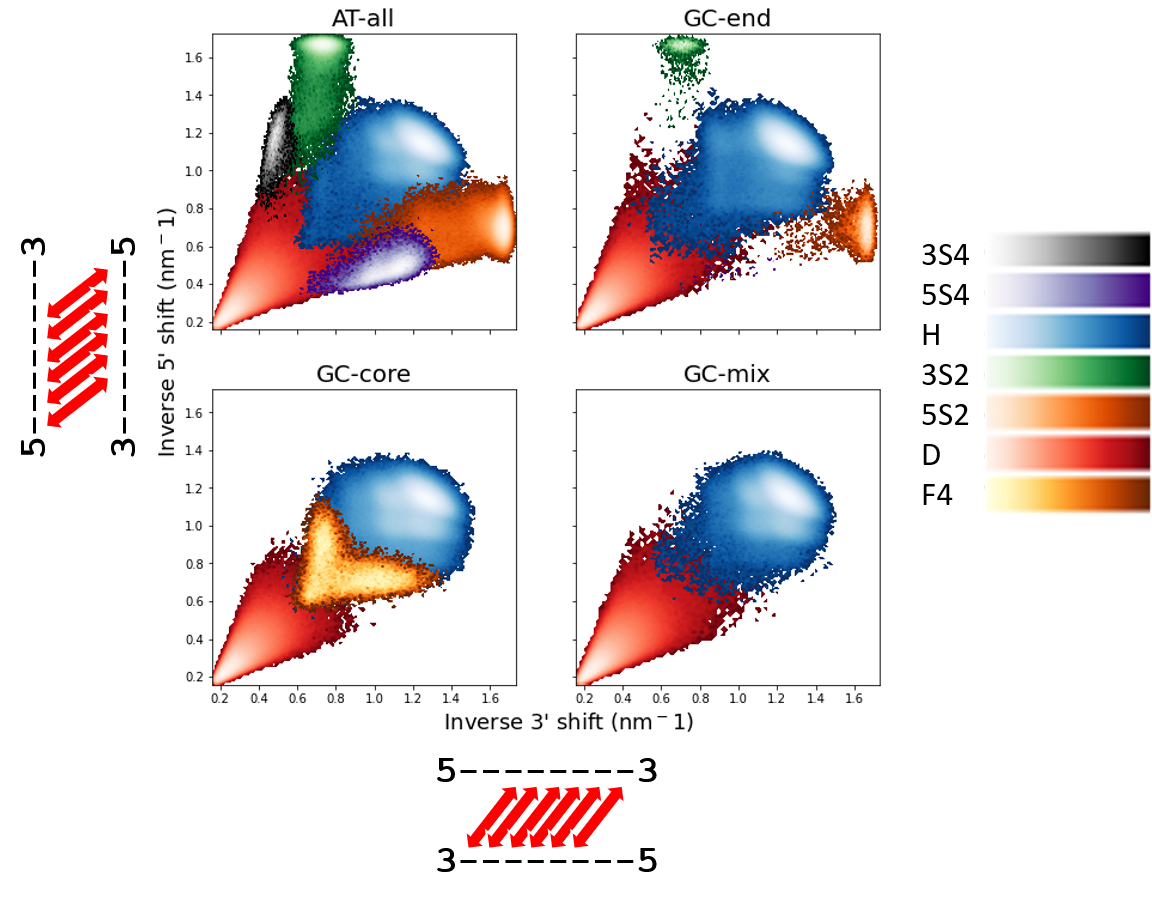
\includegraphics[width=150mm]{cover_letter/revision_figures/macrostate_colors_FES.png}
        \caption{Free energy surface of each macrostate and sequence combination. The x and y axes correspond to the reciprocal mean distance between 2-base-shifted base pairs in the 5$\prime$ and 3$\prime$ directions, respectively. These distances are visualized by the corresponding red arrow representations. Color maps define both the macrostate identity and relative free energy of a region within that macrostate, lighter regions correspond to lower free energy.}
        \label{fig:macrostate_colors_FES}
	\end{center}
\end{figure}

With regard the molecular renderings shown in figures 2A and 2C, these were chosen from microstates with the highest probability of being assigned to their corresponding macrostates. Accordingly, they should correspond to structures  that are most representative of that macrostate as whole. As the reviewer points out, it is unclear how these selected microstates were defined in the main text, and we include the following addition to section 3.2 to make this point explicit:

``We present these seven macrostates in Fig. 2a along with schematic and cartoon renderings of representative microstates contained within each of these macrostates. \rood{Molecular renderings were sampled from microstates with the highest probability of being clustered into their respective PCCA+ macrostates and should therefore reflect the macrostate population as whole. A more detailed representation of macrostate membership is shown in supplemental figure \noteg{add supplemental reference here}''}

\textcolor{blue}{1)      It is unclear how five datasets were selected used for cross-validation in the SRVs (P. 10 L. 43). One would naively think a 50:50 split of a single trajectory would result in only one dataset. A bit more detail could be provided here.}

\textbf{Author Reply:}   Five-fold cross-validation was conducted by randomly partitioning 40 independent trajectories into two sets of 20. In this way, all data is included in each fold but with distinct test/train sets. This approach prevents rare events from being left out of small validation sets and was used in our previous study, where one long trajectory was broken up into 100 \citep{Sidky2019High-ResolutionVAMPnets} smaller trajectories for training. We have  clarified this in the text by adding the following sentence to section 2.1: 

We guarded against overfitting using five-fold cross-validation in which we divided the trajectory data into 50:50 training:validation splits \rood{such that random combinations of 20 trajectories were partitioned into each set}.\citep{Sidky2019High-ResolutionVAMPnets}

\textcolor{blue}{2)      For the validation of embedding dimensions (P. 11 L. 3), it is hard to judge the presence of a kink at 5D in the AT-all sequence since only a maximum of 6D is shown in Figure S1. Could a few additional dimensions be provided?}

\textbf{Author Reply:}   We agree that it is more difficult to see the kink for the AT-all sequence than the other sequences. As suggested by the reviewer, we added two additional modes to the cross-validation procedure showing this kink after five modes and have updated the AT-all subplot of Figure S1 with the panel shown in Figure \ref{fig:AT-all_crossval}.

\begin{figure}[ht!]
	\begin{center}
        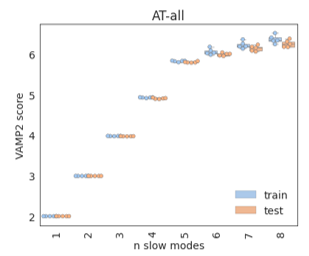
\includegraphics[width=75mm]{cover_letter/revision_figures/AT-all_added_modes.png}
        \caption{Cross-validation for the AT-all sequence with two additional modes to show the presence of a kink in the VAMP-2 score after the fifth mode.}
        \label{fig:AT-all_crossval}
	\end{center}
\end{figure}

\textcolor{blue}{3)      The values associated with the “slow” and “fast” rates appear to be inverse quantities, but this is not mentioned in the text (P. 14 L. 44).}

\textbf{Author Reply:}   The reviewer is correct that the rates have units s$^{-1}$ and describe the inverse of the experimental timescales shown on page 14. We agree that the sentence on (P. 14 L. 44) in unclear in its current form and have made the following change:

``We conducted T-jump IR experiments for each DNA sequence as a function of temperature and extracted \rood{the ``slow'' $k_d^\mathrm{slow}$  and ``fast'' $k_d^\mathrm{fast}$ rates, corresponding to processes on the 10-30 $\mu$s and 70-100 ns timescales, respectively''}

\textcolor{blue}{4)      In Figure 1 the units for rates are not provided.}

\textbf{Author Reply:}   Figure 1 has been updated to include units in s$^{-1}$. In accordance with suggestions by reviewer \#3 we have also displayed the slow responses on a y-log axis, and used the finite size effect correction mentioned by reviewer \#2 to improve the fit (Figure \ref{fig:conc_correction}). \noteg{Should we include the figure here instead? Thought it made more sense in the R2 section since we are addressing a more substantial change}

\textcolor{blue}{5)      In the comparison between experiments and theory for slow and fast T-jump IR responses (P. 17 L. 9), were there any correlations between the goodness-of-fit in the calculated rates (Figure S4) and the agreement with experiments for a given system? It is hard to judge as is because the goodness-of-fit values were not provided with Figure S4.}

\textbf{Author Reply:}     We have updated all Figure S4 plots to include goodness-of-fit values determined by the $R^2$ values of log fits (Figure \ref{fig:goodness-of-fit}). We have also re-plotted these on the log axis for easier comparisons between the simulated data and fits. Although all fits are strong, it does appear that GC-core may be slightly worse than the others sequences. As the reviewer suggests, this may be a contributing factor to the weaker experimental agreement for GC-core as well, however it is difficult for us to make that claim definitely given the data. As we note in the original text, this discrepancy may also be a result of its high propensity to fray. \noteg{Not sure if we really want to go into this or update the main text?}

\begin{figure}[ht!]
	\begin{center}
        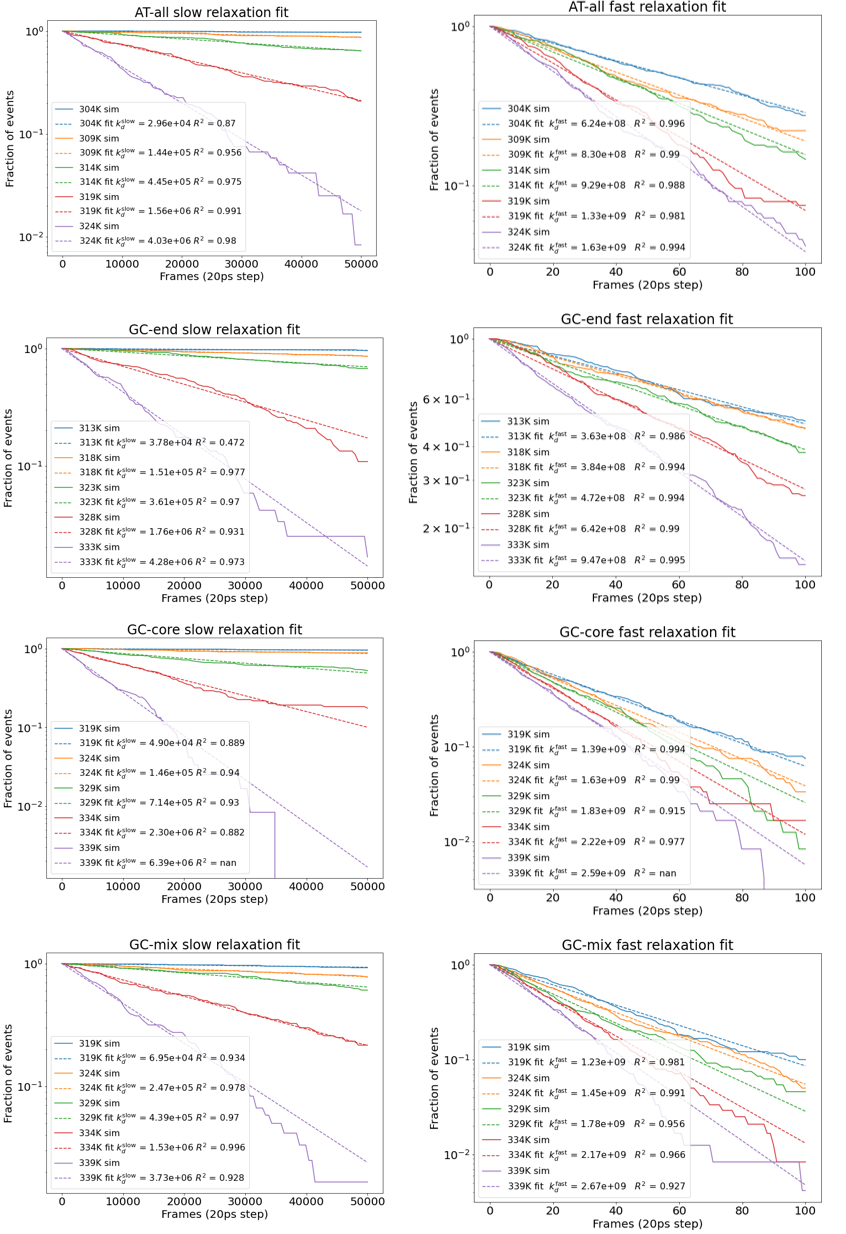
\includegraphics[width=120mm]{cover_letter/revision_figures/goodness_of_fit.png}
        \caption{Exponential fits for both slow (dissociation) and fast (fraying) response for all four sequences during ``computational T-jump'' experiments. We have updated this supplemental figure to include goodness-of-fit values determined by the $R^2$ values of log fits and plotted both the slow and fast fits on a log scale.}
        \label{fig:goodness-of-fit}
	\end{center}
\end{figure}

\textcolor{blue}{6)       The authors chose to compute the temperature jump relaxation rates from fits to quantities obtained directly from the MD simulation. However, it is not clear why the authors did not also compute the relaxation of observables from estimated Markov state models following (P. N. A. S. USA. 2011;108(12):4822-4827). This approach has also been previously used to compare kinetics obtained from Markov state models with other spectroscopic temperature-jump based experiments in DNA (J. Phys. Chem. B. 2019;123(10):2291-2304.) and RNA (J. Chem. Theory Comput. 2017;108(2):926–934) oligomers which should be mentioned. If possible, it would be interesting to compare or discuss the differences between their approach and these previous approaches.}

\textbf{Author Reply:}   The reviewer raises an important point regarding previous methodologies that have been developed to directly recapitulate experimental relaxation rates from MD-derived MSMs.

\noteg{This paragraph may not be necessary}
We have since experimented with some of these techniques using built-in PyEMMA functions, and although the results are interesting, they do not provide the most informative analysis of these particular dynamics or a strong experimental connection. We believe this is the case for the following reasons: i) shifting dynamics occur on timescales approaching that of dissociation and ii) shifting populations are small in amplitude relative to fraying and full dissociation and iii) a shifting signal is difficult to interpret experimentally without a more advanced technique such a as isotope labeling. \noteg{check with Brennan here} The combined result of these effects is that shifting dynamics are thought to make small contributions blended with the slow dissociation response. We support this hypothesis with data shown in Figure \ref{fig:responses_all}) \noteg{not sure how much to go into here}.

\begin{figure}[ht!]
	\begin{center}
        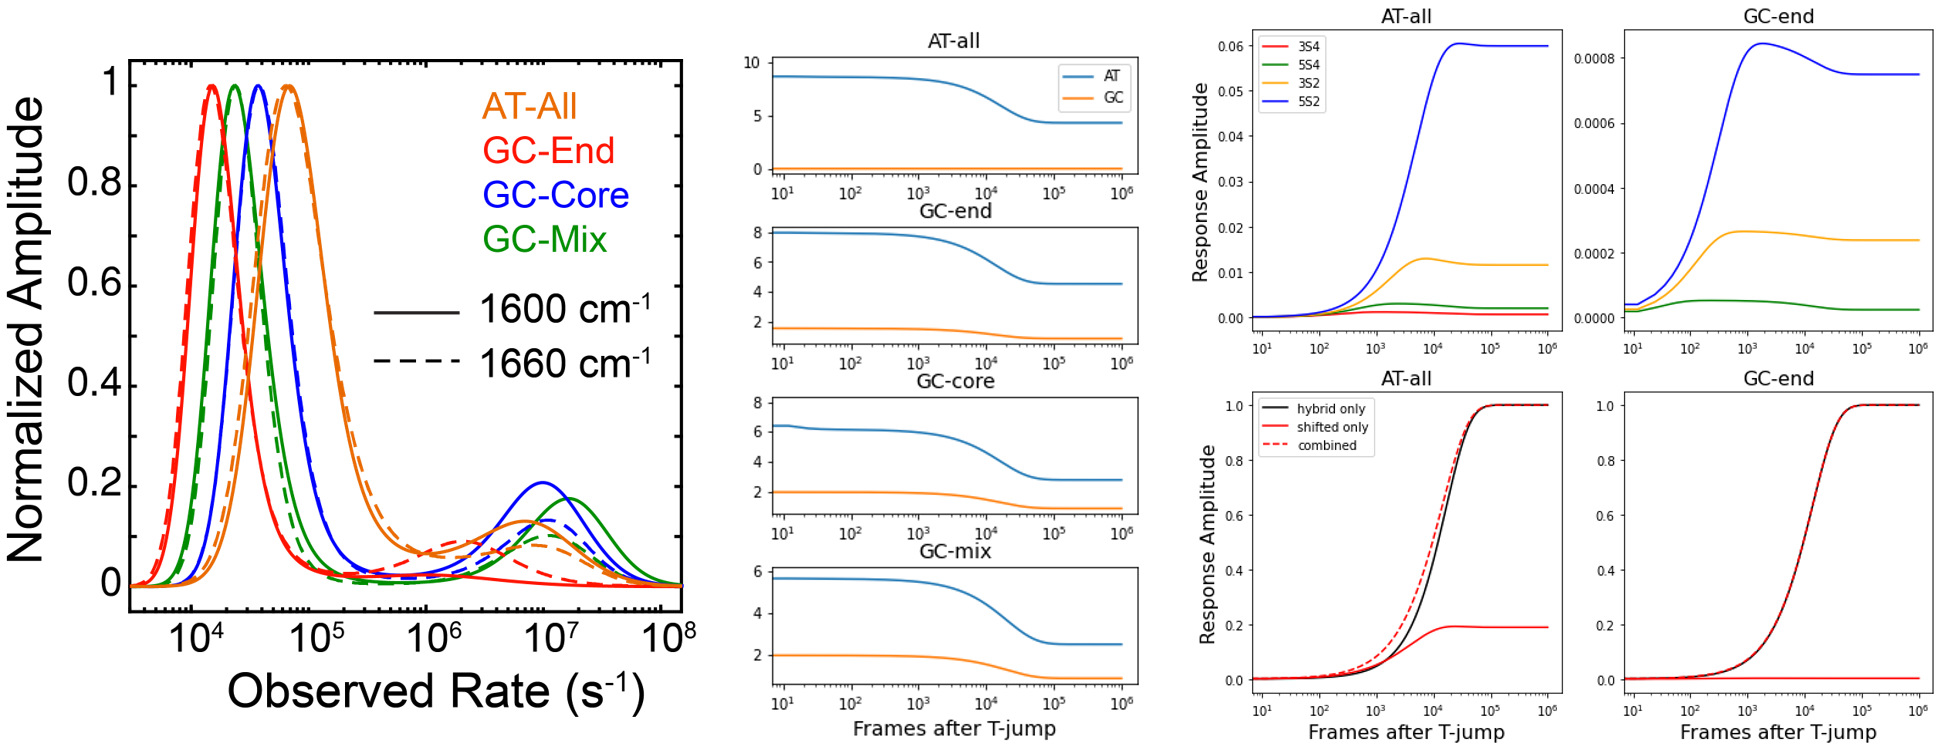
\includegraphics[width=150mm]{cover_letter/revision_figures/responses_all.png}
        \caption{a) Experimental rate representations for each sequence. Both the 1600 cm$-1$ corresponding to A,T dynamics and 1660$-1$ corresponding to G,T dynamics are shown. b) Simulated relaxation using MSM built from each sequence. An A:T and G:C response are calculated based on the distance between available WC pairs. c) Change in response when factoring in shifting motions. Because shifting is low in amplitude and occurs on timescales approaching full dissociation, the response is not expected to be clearly discernible experimentally.  \noteg{need more description here, but not sure how much of this to include} }
        \label{fig:responses_all}
	\end{center}
\end{figure}

% Can also describe fraying issue
% The appraoch in PNAS assumes that the dynamical observable can be captured by a markovian lag time
The second problem we encountered with the MSM relaxation approach is that it does not adequately describe fast-termini fraying. As discussed in section 3.1, the experimental fast responses is thought to corresponds to single base fraying of (mostly A:T) termini. This is a process that occurs even faster in simulation as shown by our derived acceleration factor. We found that although fraying does occur for each sequence, this process cannot be captured by a Markovian lag time. On the other hand, multi-base fraying observed in GC-core is slower and corresponds to the second leading slow mode for that sequence. As shown in Figure \ref{fig:responses_all}b, we only see a distinct fast response for GC-core despite the fact that termini fraying is occurring in each sequence (as demonstrated by Figure 1 in the main text). 

In addition to the issues discussed above, the main reason that we extracted responses directly from MD simulations was that effects of coarse graining, concentration, salt, etc. were unknown and could not be accounted for at a single temperature. For the slow response in particular,  timescales have an exponential dependence on temperature which could not be sufficiently standardized between experiment and simulation. Furthermore, generating equilibrium simulation data over a range of temperatures for each sequence was computationally prohibitive, prompting our decision to run an ensemble of shorter simulations at each temperature.

The additional references cited by the reviewer highlight important related work and should be included \citep{Noe2011DynamicalExperiments, Pinamonti2017, Remington2019MolecularKinetics}. Although we discussed our work's connection to (J. Chem. Theory Comput. 2017;108(2):926–934)\citep{Pinamonti2017} in the introduction, we did not originally reference it with respect to relaxation rate simulations. We do believe that our work is quite distinct from these previous studies, given that much smaller RNA oligonucleotide systems were investigated. Furthermore, the RNA studies were either lacking experimental data or compared against older data which suffered some experimental flaws. This highlights the difficulty in making strong experimental comparions for oligonucleotide systems using MSM relaxation techniques alone.

We have added the following text to section 3.1 make some of these difficulties more explicit and qualify our approach:

\noteg{Not totally sure where do put this, maybe end of first paragraph of 3.1 or at the end of that section?}

\rood{"Previous studies have used a dynamical fingerprinting approach \citep{Noe2011DynamicalExperiments} to compute rates from MSMs. These techniques were used to study base stacking dynamics in 2-4 base RNA oligomers \citep{Pinamonti2017, Remington2019MolecularKinetics} and some attempts were made to compare against experiment. However, Limitations in all-atom force fields and potential experimental artefacts have made strong comparisons difficult to achieve for oligonucleotide systems \citep{Pinamonti2017}. We tried applying these techniques with our SRV-MSMs as well, but found that i) termini fraying timescales were too fast for a Markovian lag time and ii) coarse-graining effects could not be properly standardized between experiment and simulations at a single temperature. This motivated us to directly analyze responses from simulation data over a range of temperatures."}

\begin{shaded}
\textbf{Response to Reviewer \# 2}
\end{shaded}

\textcolor{blue}{This paper reports simulation results on the hybridization and dehybridization mechanisms near to the melting temperature of a number of short DNA sequences, and accompanying temperature jump IR experiments. The sequences are chosen to have a repeating AT motif that potentially allows relatively stable out-of register duplex states, with a focus being on how these states are disrupted, by the presence of GC base pairs. The authors show that the introduction of just 2 appropriately-positioned base pairs can change the kinetics to a simple two-state behaviour from one in which multiple states contribute.}

\textbf{Author Reply:}   We thank the reviewer for their comments. \noteg{need to say anything here?}

\textcolor{blue}{I found this an interesting study that nicely illustrated some of the potential effects of sequence on (de)hybridization mechanisms. However, I found the results unsurprising, and these types of effects have been previously explored in the literature. Although I can't therefore recommend publication in JACS, I think it would be very appropriate for one of the more specialized ACS journals.}

\textbf{Author Reply:}  We are glad that the reviewer finds our results interesting, and we acknowledge that there is precedent in the literature for the states and mechanisms that we discuss.  Indeed, although similar dynamics have been identified previously, the transition probabilities between states and sequence-dependent affect on these transitions has not been identified and quantified. As suggested by reviewer \#2 and later by reviewer \#3, we have updated several introductory sentences to specify that the transition network between states reflects is significance of this work rather than the discovery of the states or mechanisms themselves

\noteg{focus more on transition probabilities and not just states? See Reviewer \#3.10 comment:}

\noteg{I think we do a pretty good job of this here:}

``Out-of-register ``shifted'' base paired structures \citep{Flamm2000RNAResolution, Romano2013DNADependence, Hinckley2014Coarse-grainedEffects, Maciejczyk2014DNAModel, Araque2016LatticeCooperativity, Xiao2019} and frayed structures \citep{Zgarbova2014BaseRNA, Nonin1995TerminalFraying, Nikolova2012ProbingSimulations, Andreatta2006UltrafastHelix} stand as candidates for metastable states with the potential to mediate substantial deviations from all-or-nothing behavior, but the degree to which these states are kinetically relevant is difficult to determine experimentally and is likely to be highly sequence-dependent.''

\noteg{Add some more changes below?}

``Consistent with previous studies, \citep{Hinckley2014Coarse-grainedEffects,Romano2013DNADependence,Araque2016LatticeCooperativity} we find the degree of repetitiveness in the sequence -- and therefore the kinetic accessibility and thermodynamic stability of out-of-register shifted states -- leads to richer dynamics populated by a diversity of long-lived metastable states. Our data-driven modeling and analysis rigorously quantifies these behaviors and furnishes accurate predictive models of the hybridization/dehybridization rates, dynamical pathways, and metastable states. Specifically, we demonstrate that disrupting repetitive stretches of A:T bases by placement of interrupting G:C base pairs enables us to tune the landscape from rich six-state to simple two-state ``all-or-nothing'' behavior, and the specific location of the interrupting pair can be used to modulate the stability of long-lived frayed states.''

\textcolor{blue}{One limitation of the study is its reliance on``brute-force'' simulations (rather than using advanced sampling/rare-event techniques) to probe the transition. This means that systems of very high concentration (7 M) and temperatures close to the melting point have to be used, which are probably not the conditions of most interest.}

\textbf{Author Reply:}    We appreciate the reviewer raising this point, and we believe that more discussion is required to motivate our choice of unbiased simulations in this work. 

The principal reasons that we performed brute force simulations were that we observed strong experimental agreement and obtained adequate sampling on the ms scale without needing to bias the system.  Indeed methods just as transition path sampling and forward-flux sampling have been successful in elucidating hybridization kinetics \citep{Sambriski2009, Hinckley2014Coarse-grainedEffects, Jin2019}, however these methods do rely on some knowledge and manual specification of relevant states or collective variables \emph{a priori}. In contrast, our unbiased approached allowed us to use a fully \noteg{can we say this?} unsupervised machine learning pipeline to cluster configuration and build MSMs. To summarize these points, we have added the following to \noteg{section} of the manuscript:

\noteg{Expand on this here?}

``The effect of the applied bias upon the thermodynamics can be rigorously corrected for using standard reweighting techniques, but approaches to rigorously correct the kinetics, particularly under the conditions of high bias necessary for good sampling, are in their infancy.''

We also note that the 7 M concentration should have been 7 mM (only 3.5x higher than the 2 mM experimental concentration), and we appreciate both reviewers \#2 and \#3 for pointing out the unphysically high reported value. We have updated this change in the manuscript in section 2.5:

``A single pair of self-complementary sequences were placed in a cubic periodic box with side length 7.8 nm corresponding to a single-strand \rood{concentration of 7 mMol/L.''}

\textcolor{blue}{Very small points:
+ p16 line 3: "Although the 3SPN.2 model reproduces melting temperatures relatively well, we observed a systematic 4 K under-prediction relative to experiment and so we apply a universal (+4) K corrective calibration to our computational results". This sentence confused me at first. I presume you are just shifting your simulated kd slow curves to better match experiment, rather than shifting the data so that the melting temperatures agree. You may want to be more explicit as I read it as the latter at first. (Note one shouldn't expect the melting temperatures to agree as very different concentrations are being used in simulation and experiment, and one also has to correct for finite-size effects when estimating melting points from single duplex simulations (https://doi.org/10.1088/0953-8984/22/10/104102)}

\textbf{Author Reply:}   We greatly appreciate this comment and suggestion, especially in the context of questions from other reviewers regarding temperature and concentration. 

\noteg{Add a small methods paragraph to describe the temp-dependent fits? I think this would also help address reviewer \#3 confusions about the various temps used }

We have since incorporated the finite size correction for homodimers reported in  https://doi.org/10.1088/0953-8984/22/10/104102 \citep{Ouldridge2010ExtractingSimulations} when computing the slow dissociation fits. We find that the results show even better agreement with experiment, motivating us to update figure 1 with these data as shown below \ref{fig:conc_correction}. In addition, we have added the units and log scale changes proposed by reviewers \#1 and \#3, respectively.

\begin{figure}[ht!]
	\begin{center}
        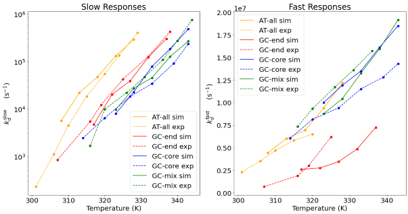
\includegraphics[width=\textwidth]{cover_letter/revision_figures/both_response_log_4K_shift.png}
        \caption{Updated figure 1 of the main text. We made three changes: i) adding units to both plots, ii) accounting for finite size effects when computing the slow response, and iii) displaying the slow response on a log axis. These were proposed by reviewers \#1, \#2, and \#3 respectively}
        \label{fig:conc_correction}
	\end{center}
\end{figure}

\begin{figure}[ht!]
	\begin{center}
        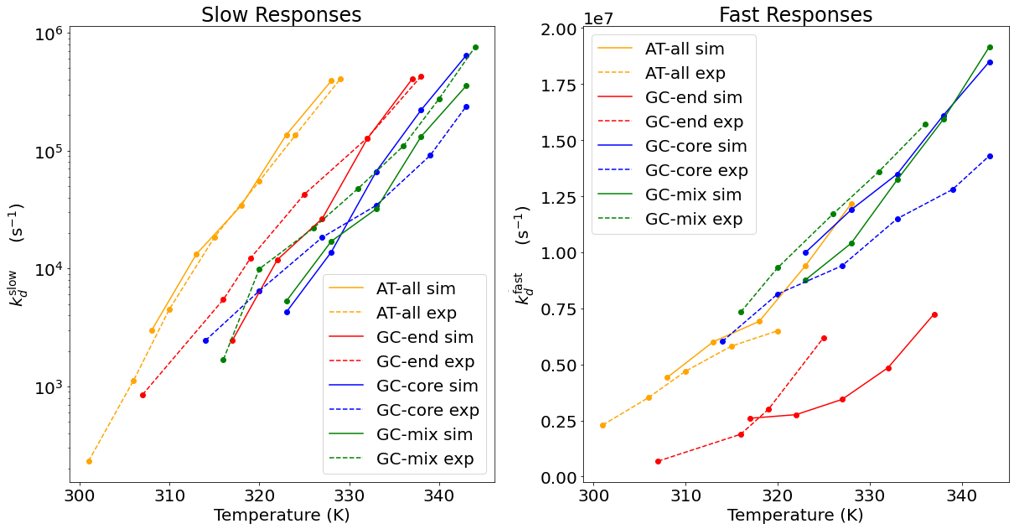
\includegraphics[width=\textwidth]{cover_letter/revision_figures/both_response_log_no_correction_4K_shift.png}
        \caption{Updated figure 1 of the main text. We added units to both plots and displayed the slow response on a log axis as proposed by reviewers \#1 and \#3, respectively \noteg{This is with no correction and the results do not look all the different (homodimer correction is less than hetero). I'm leaning towards just using this given that the temp-dependent simulations are not performed in equlibrium and the correction appears unncessary}}
        \label{fig:conc_no_correction}
	\end{center}
\end{figure}

\noteg{Everything below would only be if we choose to include the fluctuation corrections}

The following was added to the methods section to describe the fluctuation correction:

\rood{The following calculates the dimer fraction in bulk solution from simulations performed in a periodic box. We apply this to the dissociation fraction in order to better compare with the experimental slow response. We compute these values from the dimer fraction (DD) and monomer fraction (D, D).}

    \begin{equation}\label{}
    \phi = \frac{\mathrm{probability (DD))}}{\mathrm{probability (D, D)}}
    \end{equation}
    
    \begin{equation}\label{}
	f_{\infty} = (1+\frac{1}{4\phi}) - \sqrt{(1+\frac{1}{4\phi})^2 - 1}
	\end{equation}

With regard to the longer simulations used to construct SRV-MSMs, we maintain the same empirical melting temperatures so as to maximize (de)hybridization events. Although selecting a slightly lower temperature for each sequence may better approximate the bulk melting temperature, we do not expect this small shift to have a substantial impact on the sequence-dependent kinetic landscapes we have reported. Furthermore, as the reviewer indicated we are already operating at a higher concentration than experiment and would not be able to recover the exact conditions given any temperature shift alone.

\textcolor{blue}{+ p15 line 20 "beyond with" -> "beyond which"}

\textbf{Author Reply:}    This typo has been corrected.

\begin{shaded}
\textbf{Response to Reviewer \# 3}
\end{shaded}

\textcolor{blue}{Jones et al present a combined experimental and computational paper that probes the dynamics of the DNA hybridization/de-hybridization transition. Through a Markov state model analysis of coarse-grained simulation, the authors identify states that contribute to the process, and present experimental evidence to support the role of these states. In particular, repetitive sequences are observed in simulations to have a number of misaligned states that are both appreciably stable and contribute to hybridization and de-hybridization pathways as intermediates. The role of these states is diminished by base pairs that disrupt the repetitive sequence. In the special case of a sequence with a strong core and weaker extremities, metastable "frayed" states are also observed. The presence of these states is assessed experimentally trough the analysis of relaxation timescales observed in T-jump IR spectroscopy; fast relaxation is attributed to fraying equilibria, and a broader fast relaxation to an increased heterogeniety due to the presence of mis-aligned intermediates.}

\textbf{Author Reply:}   We appreciate the reviewer's detailed summary of our work

\textcolor{blue}{The paper is generally well-written, and, I believe, represents a good attempt to tackle this important process. I personally have had a manuscript "desk-rejected" by JACS on the basis that it is "too focussed on DNA biotechnology", and "primarily of interest to RNA and DNA chemists". The same statements could be made about this paper. However, I disagree with the conclusion that such papers are not appropriate for JACS. I would therefore recommend publication, subject to satisfactory responses to the comments below.  }

\textbf{Author Reply:}   We are pleased that the reviewer finds the paper both well-written and of high significance to JACS readers.

\textcolor{blue}{1.   I was frequently confused as to the temperatures used in the experiments and analysis. At one point, it is noted that simulations are performed at melting temperatures. However, simulations are actually performed at a range of temperatures and it isn't always clear when looking at a figure which temperatures were used for simulation, NN model comparison or experiments (see eg. Figs 2 and 3 and 5). I would recommend noting the temperature used to obtain the data in each case.}

\textbf{Author Reply:}   This is a good comment that requires some clarification in the text. We should be more explicit that the MSM data was all acquired at sequence-specific melting temperatures, but the experimental validatoin in 3.1 was performed over a range of temperature in experiment and simulation. 

\noteg{we don't really have a methods section on the temp-dependent simulations, maybe this should be added to 2.1.1 address this comment and a question from reviewer \#2? Alternatively we could just add something like this to the intro in addition to another sentence or two?}

"We validate the new computational models of hybridization/dehybridization dynamics developed in this work against new experimental data \rood{over a range of temperatures} and reinterpret our prior experimental observations in light of the new computational understanding."

\textcolor{blue}{P7 line 13 - surely these simulations were not really done at 7M? That sounds impossibly dense.}

\textbf{Author Reply:}2.    We appreciate the reviewer pointing out this error in our reported units. The value should be 7 mM, not 7 M as shown in the below calculation. This has been corrected in the manuscript. 

    \begin{equation}\label{}
	\frac{2 \mathrm{\:oligos}}{\mathrm{box\:volume}} = \frac{2}{7.80\mathrm{\:nm}^3} = 
	\frac{3.32 \times 10^{-24} \mathrm{\:moles}}{4.75 \times 10^{-25} \mathrm{\:m}^3} = 
	6.99 \frac{\mathrm{moles}}{\mathrm{m}^3} \approx 7\mathrm{mM}
	\end{equation}

\textcolor{blue}{3.  The authors repeatedly refer to "slithering" mechanisms for rearrangement. I believe this is unfortunate. In the context of the 3SPN model, the "slithering" term was first introduced in Ref. 49 by Sambriski et al, and describes two helical single strands sliding along each other. As noted by Hinckley et al in Ref 18, that mechanism is largely an artifact of the form of the potential in 3SPN.1. The rearrangement mechanism in 3SPN.2 is more of a "defect diffusion", analogous to the "inchworm mechanism" previously identified in the oxDNA model (ref 52 - note, the author list for this reference is wrong). Given this context, it seems unnecessarily confusing to talk about "slithering".}

\textbf{Author Reply:}    We share the reviewer's concerns with using ``slithering'' to describe a process that would be more appropriately called ``defect diffusion'' or the ``inchworm mechanism.`` In the manuscript, we made the effort to only use this term in reference to studies that were focused on this processes and described it as such -- namely refs 17 and 49 \noteg{update these after adding ref}. In our revisions, we have removed the term from the introduction so that it now reads as follows:

``An energy disconnectivity graph-based approach was used to interrogate the differences in hybridization rates and mechanisms between GGGGGG and GCGCGC hexamers to reveal strong deviations from ``all-or-nothing'' behaviors and the importance of zippering and \rood{out-of-register diffusion mechanisms.~\citep{Xiao2019}''}

The term is also referenced on page 27 but enclosed in quotation marks to show that we are using terminology from ref 17 and not implying that this processes defines the mechanisms we observe in this work.

\noteg{No change below yet. Could add quotes to the second instance of slithering or just remove the word entirely? Not sure if either is necessary}

\rood{``Out-of-register states for 5$^\prime$-GCGCGC-3$^\prime$ hexamers were identified as deep kinetic traps along the hybridization pathway and ``slithering'' through these states did not provide a significant hybridization pathway compared to an alternative ``zippering'' mechanism. (In contrast, out-of-register slithering and in-register zippering served as two parallel pathways for hybridization of 5$^\prime$-GGGGGG-3$^\prime$.)'' }

We also appreciate the reviewer pointing out the incorrect author list in ref 52, and we have fixed the issue.

\textcolor{blue}{4. P15: I am a bit surprised that a separation of 1.3nm between the central base pairs is enough to guarantee strand separation, given that frayed end can separate by 1.3nm when the core is intact. Can the authors verify that all their duplexes had truly separated at this point?}

\textbf{Author Reply:}   This a good point of clarification. Given the importance of the core contacts during duplex dissociation, we found that any cutoff value from 0.8 nm - 2.5 nm is indicative of full dissociation and yields very similar results when calculating the slow response. On the other hand, the fraying cutoff should measure complete termini dissociation without requiring multiple bases to dissociate and thus should be chosen more carefully. 

To demonstrate the flexibility of this parameter, we show the slow response from Figure 1a with dissociation cutoffs at 1.3 nm to 2.0 nm. These plots, shown in Figure \ref{fig:compare_cutoffs}, also incorporate the finite size correction proposed by reviewer \#2 and log y-axis suggested in the next comment.

\begin{figure}[ht!]
	\begin{center}
        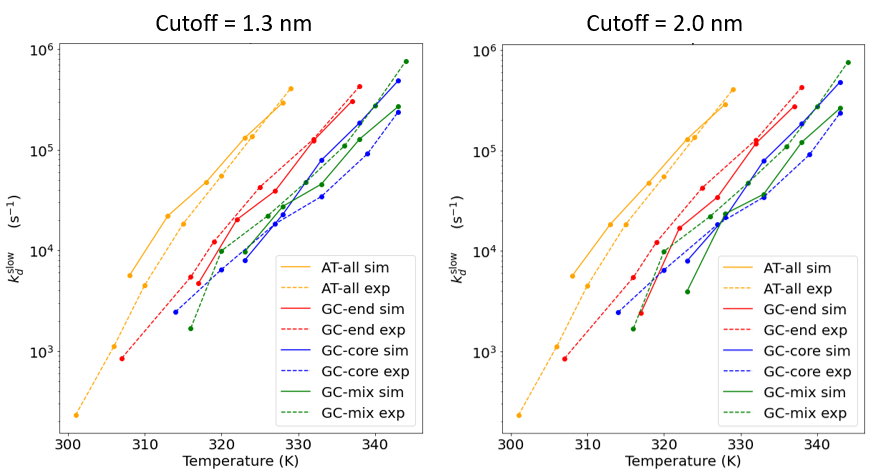
\includegraphics[width=\textwidth]{cover_letter/revision_figures/slow_response_compare_cutoff.png}
        \caption{Comparing the experimental slow response when increasing the cutoff parameter from 1.3 nm to 2.0 nm}
        \label{fig:compare_cutoffs}
	\end{center}
\end{figure}

\textcolor{blue}{5. The authors refer to "exponential" increase in Fig. 1. However, it's hard to see that an increase is exponential by eye unless the data is plotted on a log scale.}

\textbf{Author Reply:}   We agree with the reviewer that a log plot is an optimal representation of the temperature-dependent slow responses. We have made this change to to Figure 1 which has been also been shown above \ref{fig:conc_correction}.

\textcolor{blue}{6. Do the authors have any data on the scaling of k\_hybridization with T? In experiment, rates appear to increase with temperature (albeit with a much weaker dependence than de-hybridization rates). Simple "nucleation and zipper" models would predict the opposite, as does the oxDNA model (see ref 52).}

\textbf{Author Reply:}   We are interested in temperature and sequence affects on  k\_hybridization and exploring a some future work in this vein. Indeed, it is possible to use similar methods to investigate the hybridization process, however these calculation require much greater computational expense in order to gather adequate statistics. As this section served more as a validation for the model’s ability recapitulate experimental responses, we do not think this work is in scope of this work. Furthermore, the k\_hybridization values gathered by T-jump are significantly less reliable than k\_dissociation as the system cools back down and timescales approach the millisecond regime. \noteg{check with Brennan on this}

\noteg{can cite some experimental work here, but the trend they describe here is not really correct}

\textcolor{blue}{7. The authors could explain a bit more carefully (perhaps in the SI) how they handle the multiple nearest-neighbour states that correspond to their microstates (eg. F4 clearly involves more than one NN configuration).}

\textbf{Author Reply:}   \noteg{Brennan working on this}  NN calculations only explicitly considered configurations where four base pairs are entirely unbound on either side, and the rest are fully bound. The analysis below adds configurations with partial fraying on one side to better treat the diversity of microstates present in F4 (Figure \ref{fig:F4_microstates}).

\begin{figure}[ht!]
	\begin{center}
        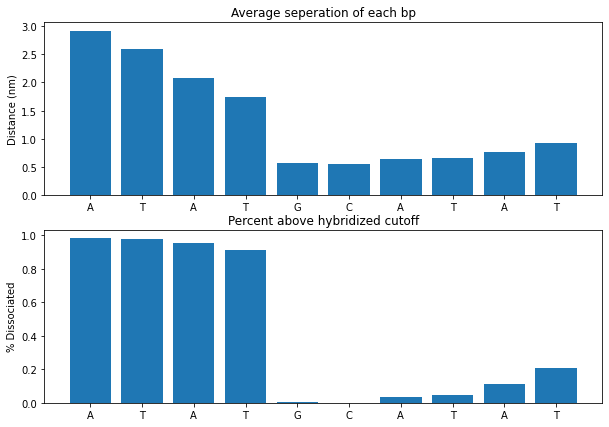
\includegraphics[width=\textwidth]{cover_letter/revision_figures/F4_microstates.png}
        \caption{Microstates distribution within the F4 macrostate. Fraying in the permutable up/down direction is symmetrized such that all frayed ends are on the left and all bound ends on are the right. Panel B shows the percentage of distances greater than a 1.3 nm cutoff, where 21\% of states have at least one base paired frayed and 11\% of states have at least two base pairs frayed. \noteg{Brennan calculating how the inclusion of these states affects the estimated free energy.}}
        \label{fig:F4_microstates}
	\end{center}
\end{figure}

\textcolor{blue}{8. I don't understand how the population of F4 could be >50\% that of H for the GC-core system, when the free energy of F4 is reported as > 5kJ/mol. My back-of-the-envelope maths predicts a ratio of 8:1 for a 5kJ/mol gap. Incidentally, 8:1 is roughly the ratio I got from running the configurations through NUPACK.}

\textbf{Author Reply:}   We appreciate this comment, and we feel that it highlights some possible confusion regarding the log population plot shown in Figure 2. Indeed, it may appear that the F4 state is >50\% that of H for the GC-core, however it is only about 1\% of the of H. We have decided to keep the log plot in order to capture small populations of shifted and frayed states, however we had added the following lines to the main text figure 2 caption:

``Histograms reporting the number of the $10^7$ total frames within the 1 ms of simulation trajectories observed to occupy each of the seven macrostates, corresponding to our numerical estimates of the equilibrium occupancy probabilities. Uncertainties are calculated across 100 MSMs using a Bayesian MSM estimation are reported for each bar and are very small compared to the total counts. \rood{Values are reported on a log y-axis to properly visualize less low-population states}'' \noteg{maybe this is too condescending}

\textcolor{blue}{9. Is the MSM model explicitly constrained to obey detailed balance? The numbers that come out seem consistent with detailed balance - forward and backward trajectories at the same T essentially look the same (they're equally likely to go through intermediates). This should be a feature of the MSM, but it's unclear to me whether it's hard-coded or just arises naturally in the coarse-graining.}

\textbf{Author Reply:}    The reviewer raises a good point regarding the assumptions made during MSM construction. We use the reversible Bayesian MSM framework described here \url{http://www.emma-project.org/latest/api/generated/pyemma.msm.BayesianMSM.html} which enforces detailed balance. This is an important point which we have made explicit in section 3.4:

``In addition to thermodynamic stabilities, the macrostate MSM also furnishes quantitative and interpretable predictions of hybridization and dehybridization pathways and mechanisms. \rood{It should be noted that because we are using a reversible MSM framework, detailed balance is enforced by construction.''}

\textcolor{blue}{Relatedly, some of the discussion of the hybridization and de-hybridization pathways in non-repetitive sequences seems to ignore this fact. In these equilibrium simulations, hybridization trajectories played in reverse should be statistically indistinguishable from de-hybridization trajectories. I don't think anything that's said is wrong, per se, but it might be worth considering how the contrast between "nucleation and zippering" and "fraying-peeling" is consistent with the symmetry in the pathways.}

\textbf{Author Reply:}  \noteg{Do we want to change this terminology? or clarify? Fraying-peeling is effectively the reverse of nucleation-zippering. If we imply that they are distinct processes, then the reviewer is correct that it undercuts the reversible MSM assumption we make when looking at the other sequences. A proposed addition is below:}

`` In dehybridization, we observe fraying on the two-base AT-tails on one or both sides of the duplex followed by rapid dissociation of the central WC base pairs. Qualitatively, we observed some short-lived states composed of two to four native WC base pair contacts immediately before full dissociation occurs, but, in contrast to the F4 state we observe in GC-core, these conformations do not constitute a metastable state within our MSM nor do they tend to reform intact duplexes. \rood{These dissociation dynamics are consistent with a ``fraying-peeling'' dehybridization mechanism.\citep{Wong2008TheSimulations, Perez2010Real-timeUnfolding, Zgarbova2014BaseRNA} which can be thought of as the analogous reverse process to nucleation-zippering. Indeed, the qualitative similarity between the forward and reverse process suggest detailed balance is obeyed and that our reversible MSM analyses are well-founded.}'' \noteg{I know this doesn't sound very good, but want to make sure this is what the reviewer is getting at.  Also, should we just get rid of citations when quoting from the main text?}


\textcolor{blue}{10. I think some of the characterisation of the "all or nothing" picture is a bit misleading. The two state model of duplex formation is really a thermodynamic model, based on the assumption that the ensemble of hybridized and de-hybridized states look very different and are separated by a large barrier. This model is perfectly consistent with the transition between the two ensembles involving a complex network of metastable states. Indeed, as the authors note on line 3 of p4, a number of previous authors have considered what such states might look like, particularly for repetitive sequences. The authors' primary contribution here is not proposing that these states exist for the first time, but trying to tie together evidence from simulation and experiment to describe them.}

\noteg{The ``all-or-nothing'' comment is an important point. Brennan had cautioned using this term necessarily synonym for ``two-state'' and the reviewer seems to be making the same point. There are 11 instances of ``all-or-nothing'' in the main text, and it is often used in conjunction with ``two-state all-or-nothing.'' I think we may want to consider removing most of them, but we should probably word this carefully.}

\textbf{Author Reply:}   We appreciate the reviewer's helpful suggestion to highlight the role of macrostates rather than the identification of states themselves. We have updated some introductory language (in response comments from reviewer \#2 as well) to better communicate the novelty of the kinetic network:

\noteg{Same change as used above in response to \#2 wrt to better introductory language. Maybe some addtions in the main text or conclusions as well?}


\textcolor{blue}{11. Related to the above, the references on line 3 of p4 should probably also include Ref 52, where a similar analysis of metastable states in a repetitive sequence is performed (for a different coarse-grained model) and [Flamm, W., Fontana,J.M., Hofacker, I.L. and Schuster,P. (2000) RNA folding at elementary step resolution. RNA, 6, 325–338] where a defect diffusion mechanism is proposed.
}

\textbf{Author Reply:}   We agree that the reviewer's suggested additions are pertinent and provide the interested reader more context into shifted states and their associated mechanisms. We have included both references in the following section: \noteg{do we actually need to paste the complete sentence if we're just adding references?}

``\rood{Out-of-register ``shifted'' base paired structures \citep{Flamm2000RNAResolution, Romano2013DNADependence, Hinckley2014Coarse-grainedEffects, Maciejczyk2014DNAModel, Araque2016LatticeCooperativity, Xiao2019}} and frayed structures \citep{Zgarbova2014BaseRNA, Nonin1995TerminalFraying, Nikolova2012ProbingSimulations, Andreatta2006UltrafastHelix} stand as candidates for metastable states with the potential to mediate substantial deviations from all-or-nothing behavior, but the degree to which these states are kinetically relevant is difficult to determine experimentally and is likely to be highly sequence-dependent.''

\textcolor{blue}{12. The reasoning behind why the broader relaxation spectrum is indicative of misaligned states was not that clear to me. Why would "elevated" fraying cause a broader response? Wouldn't it also, then, be broader for CG-core, which has elevated fraying? It seems to me that the argument is more along the lines of the heterogeneity of the configurations leading to heterogeneous dynamics, and hence a broader relaxation profile. But I am no expert on this technique.}

\textbf{Author Reply:}   The reviewer makes a good comment on our choice of language used to described the stretched AT-all response. 

In its current form, the section may mislead the reading into thinking that an elevated fraying response alone would cause a broader fast response. As the reviewer indicates, this would would suggest that GC-core might have the most stretched response. Our hypothesis, rather, is that differential fraying behavior from an ensemble of shifted states will stretch the fast response relative to fraying from only intact duplexes. We believe that the reviewer's apt suggestion ``heterogeneity of configurations leads to heterogeneous dynamics'' expresses this idea much more clearly and we have integrated it into the final paragraph of section 3.7. We have also 

% Should not use "elevated" response here but rather put the emphasis on broadening the response. (borrow lanaguage)

The latter interpretation here is correct. The key is that the response does not come from shifting itself, so it’s fraying in the shifted state that would cause the change in response. We have have updated the language in the section to better express this point. (configurational entropy)

``Nevertheless, the presence of these out-of-register shifted states in the low-temperature equilibrium ensemble prior to the T-jump step may be observable via their influence on the fast T-jump IR response attributable to fraying. Specifically, we hypothesize that the dangling ends and inert tails present in the out-of-register shifted states should promote an \rood{elevated fraying response over the course of the relaxation that is distinct from that of in-register fraying. This heterogeneity of configurations should lead to heterogeneous dynamics, manifested in the observation of a more stretched relaxation over experimental time scales of 70-100 ns.} Analysis of the MSM equilibrium distributions reveals 10.0\% of the equilibrium ensemble to reside in out-of-register shifted states 3S2, 5S2, 3S4, and 5S4 for AT-all, compared to just 0.23\% for GC-end, and 0\% for GC-core and GC-mix. It is our conjecture that a substantial population of out-of-register shifted states in the pre-T-jump AT-all ensemble should be distinguishable from the GC-end, GC-core, and GC-mix as an elongation of the fast relaxation response associated with terminal base fraying.''

\textcolor{blue}{13. How much of the code is being made available? Ideally, the initialization files for the simulations and the code used to perform the MSM analysis would be publicly available. Additionally, it would be good to publish the raw experimental data and the processing tools used to obtain the final results.}

\textbf{Author Reply:}   We agree that the data and analysis code should be made accessible for future analysis. We have uploaded input files and analysis scripts to Github ( \url{https://github.com/mrjoness/DNA_SRV-MSMs}) and  \noteg{45 GB} of featurized trajectories to Zenodo (\noteg{Zenodo link}).

\begin{shaded}
\textbf{Additional editorial edits}
\end{shaded}

\textcolor{blue}{1. Please include at least the first page for each reference citation for the following incomplete journal reference 48}

Updated

\textcolor{blue}{2. Please update the publication status of reference 70, if possible.  Providing the DOI is acceptable.}

\noteg{Does not seem like there is a submission history or DOI for this. Actually listed as a book chapter, but unclear from where. Could just remove this since most info is contained in ref 69 anyway?}

\textcolor{blue}{3. Please include publisher for the following incomplete book reference: 79.}

Updated

\textcolor{blue}{4. The TOC graphic should fit in an area no larger than 3.25 in. by 1.75 in. (approx. 8.25 cm by 4.45  cm) and should have adequate resolution and clarity. Confirm that all text is legible at this size.}

SRV axis labels were enlarged in the bottom right panel and the loss function was removed from the top right panel (Figure \ref{fig:TOC_square}). \noteg{perhaps the flattened version is more appropriate for the aspect ratio? Should we provide both? (Figure \ref{fig:TOC_long})}

\begin{figure}[ht!]
	\begin{center}
        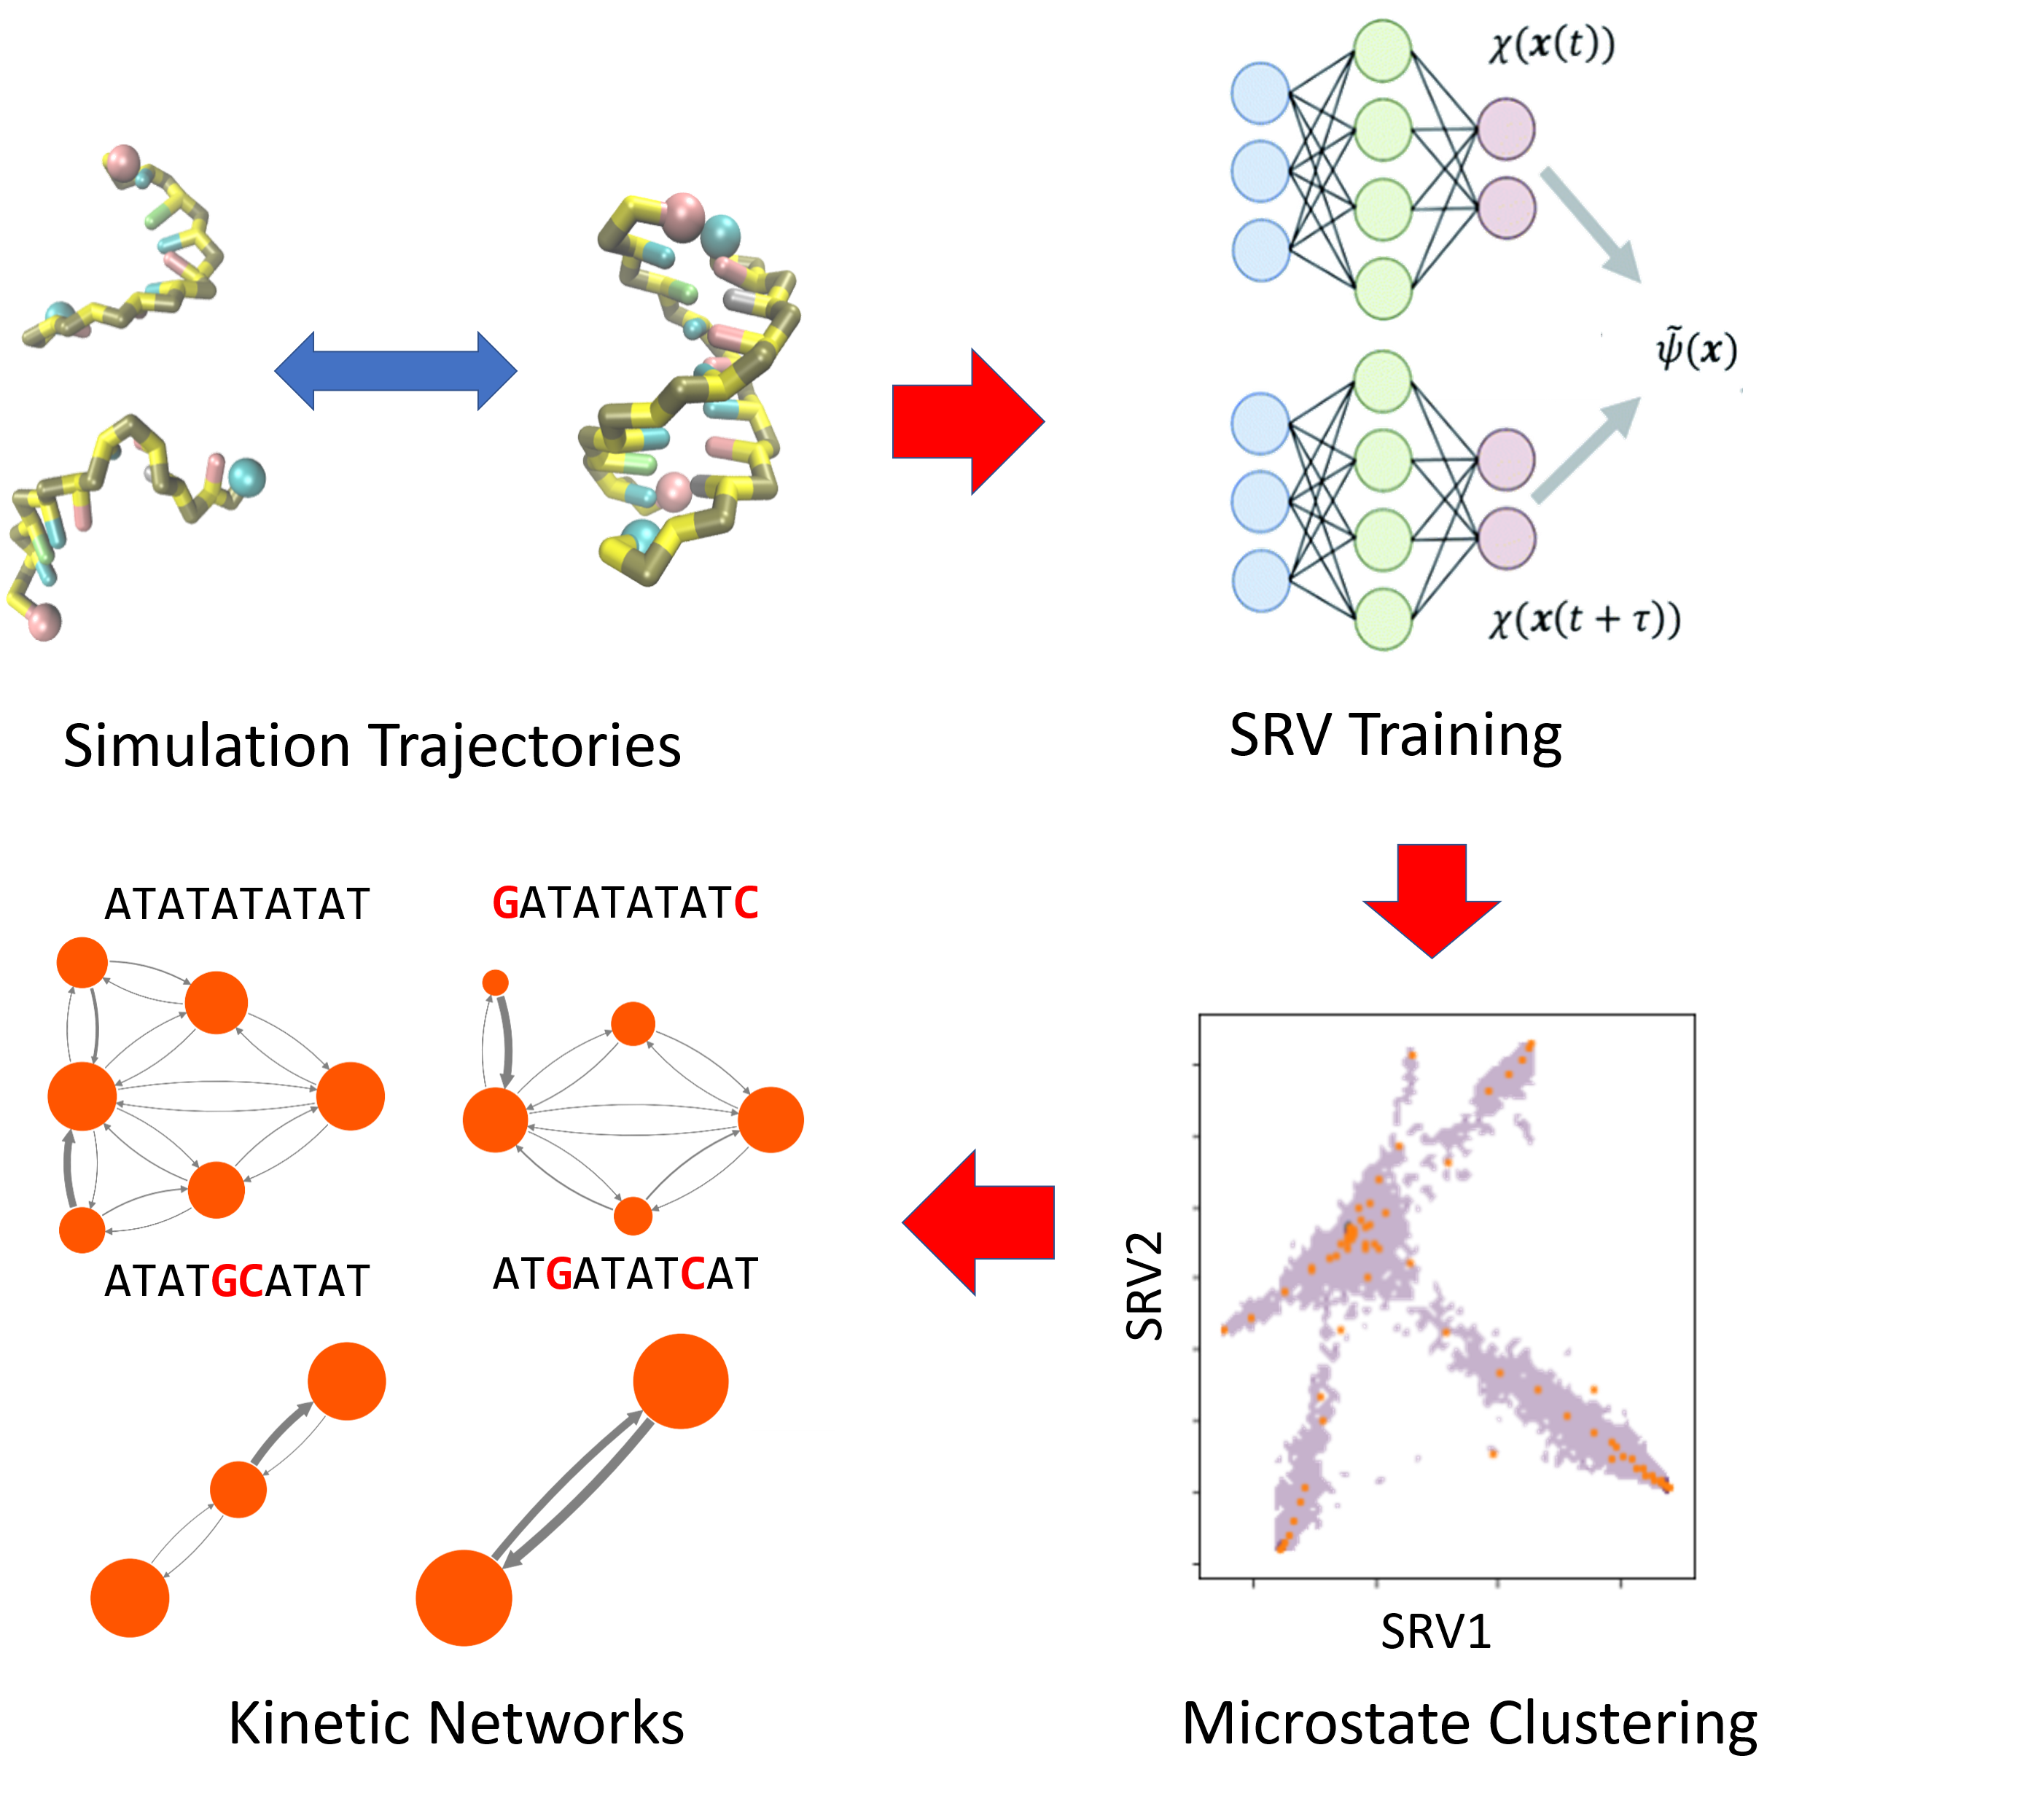
\includegraphics[width=\textwidth]{cover_letter/revision_figures/TOC_updated.png}
        \caption{}
        \label{fig:TOC_square}
	\end{center}
\end{figure}

\begin{figure}[ht!]
	\begin{center}
        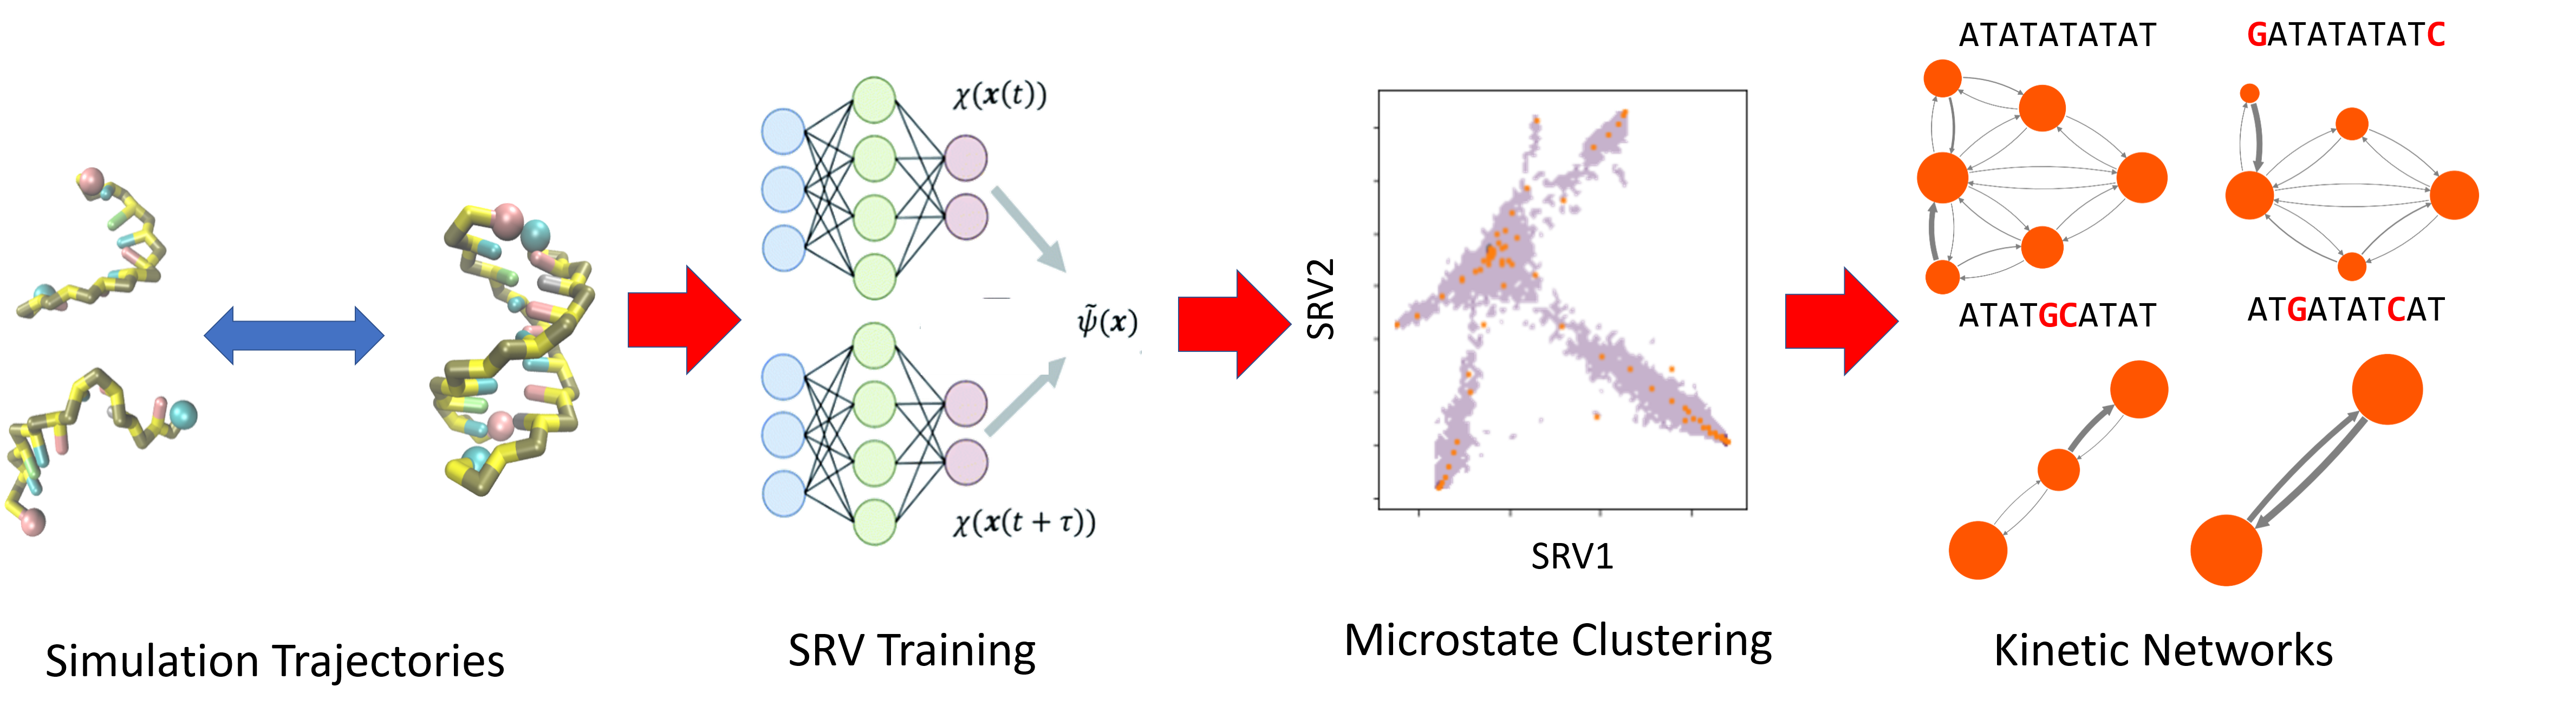
\includegraphics[width=\textwidth]{cover_letter/revision_figures/TOC_updated_long.png}
        \caption{}
        \label{fig:TOC_long}
	\end{center}
\end{figure}

\clearpage
\newpage

\bibliographystyle{achemso}
\bibliography{references_210514_abv}
\end{document}

